\documentclass[a4paper, title page, 12pt]{report}

\usepackage[utf8]{inputenc} % permet d'écrire des caractères accentués et autres trucs direct
\usepackage[T1]{fontenc} % norme T1 LaTeX
\usepackage[french]{babel} % renommage français
\usepackage{graphicx} % permet l'insertion d'image
\usepackage{geometry} % permet le redimensionnement plus pratique de la page ou la mise en "landscape" (paysage) d'une feuille
\usepackage{xcolor}
\usepackage{tikz}
\usepackage[final]{pdfpages} 
\usepackage{amsmath}
\usepackage{amssymb}
\DeclareMathOperator{\commande}{texte}

% package et définitions des en-têtes et pieds-de-page
	\usepackage{lastpage}
	\usepackage{fancyhdr}
	\pagestyle{fancy}
	\renewcommand{\headrulewidth}{1pt}
	\fancyhead[L]{\leftmark}
	\fancyhead[C]{}
	\fancyhead[R]{}
	\renewcommand{\footrulewidth}{1pt}
	\fancyfoot[C]{ÉCOLE NATIONALE SUPÉRIEURE D'INFORMATIQUE POUR L'INDUSTRIE ET L'ENTREPRISE \\ 1,  square de la résistance 91025 ÉVRY - http://www.ensiie.fr/ \\ 		\textbf{Page \thepage/\pageref{LastPage}}}


\makeatletter
\let\ps@plain=\ps@fancy
\makeatother
% des trucs pas très utiles pour ce document mais quand même !
	\title{IIAR - Rapport final du jeu de dames}
	\author{Romain EPIARD - Fabien GOUGET}
	\date{}
	
	\begin {document}
	% première page
		\begin{titlepage}

			\begin{center}

			
\includegraphics[scale=0.5]{img/Logos/logo_ensiie.png}

			\bigskip

			\bigskip

			\bigskip


			\bigskip


				\begin{large}



						\textbf{É}cole \textbf{N}ationale \textbf{S}upérieure d'\textbf{I}nformatique pour l'\textbf{I}ndustrie et l'\textbf{E}ntreprise

						\bigskip

						\bigskip
						
						\bigskip

						\bigskip

						\bigskip

						\bigskip
						
						\bigskip

					\begin{bfseries}

						\begin{tabular}{|p{10cm}|}

							\hline

							\begin{center}

								Intelligence Artificielle \\
								
								Spécifications - Jeu de dames\\

						

								\bigskip



								Année universitaire 2015-2016 \\



								\bigskip



								2\up{ème} année

							\end{center} \\

							\hline

						\end{tabular}




						\bigskip

						\bigskip

						\bigskip

						\bigskip

						\bigskip

						\bigskip

						\bigskip
						
						\bigskip
						
						\bigskip

						\begin{tabular}{l l}

							Réalisé par : & Romain EPIARD \\
										  & Fabien GOUGET \\

						\end{tabular}
						\bigskip
						\bigskip

					\end{bfseries}

				\end{large}

			\end{center}



		\end{titlepage}
		
	\setcounter{page}{1}
	\newpage

% table des matières
	\tableofcontents
	\newpage
	\section*{Introduction}
	Nous avons choisi de développer l'intelligence artificielle d'un jeu de dame. Nous allons d'abord implémenter une IA de base, comprennant un algorithme de type Min-Max, un Alpha-Beta et une Fonction d'évaluation viable. Une fois cette IA implémentée, nous voudrions implémenter une IA un peu plus poussée, avec une mémoire. Cela lui permettrait d'apprendre les coups à ne pas faire, une fois un certain point atteint. Nous pensons que le plus difficile dans l'implémentation d'une mémoire serait de définir un point de non retour, qui nous permettrait de définir si l'on doit enregistrer une partie ou non dans la mémoire de l'IA. Mais tout d'abord, il nous faut implémenter les règles du jeu.
	\newpage	
	\chapter{Projet}
	\section{Règles du jeu de dames}
	Les règles suivantes sont celles que nous avons implémenté dans notre projet. Le jeu de dames se joue sur un plateau de 100 cases (10 cases par 10 cases). Chaque joueur possède 20 pions. Il y a deux joueurs. Un des joueurs utilise les pions blancs, l'autre les pions noirs. Les pions ne peuvent se déplacer qu'en diagonale. Pour prendre un pion du joueur adversaire, il faut qu'il y ait une case vide de l'autre côté du pion à prendre.\\
	
	Pour implémenter le jeu, nous avons commencé par récupérer une I.H.M. Cette interface homme-machine a été récupérée sur internet. Ensuite, à partir de l'interface récupérée, nous avons ajouté les règles du jeu de Dames décrites plus haut. Nous avons essayé de rester fidèle le plus possible aux règles officielles du jeu de Dames. Nous avons eu quelques problèmes lors de l'implémentation du déplacement des pions. En effet, un pion qui peut prendre un autre pion est dans l'obligation de le faire. Si il peut en prendre plusieurs à la suite, il faut gérer le déplacement du pion. Et c'est la prise de plusieurs pions à la suite qui nous a posé problème. Car il fallait détecter la prise d'un pion, mais aussi détecter si une fois qu'il avait pris un pion, il pouvait en prendre d'autres, et ainsi de suite. Comme cette étape nous a posé plus de problèmes que prévu, nous avons décidé de ne pas implémenter la transformation d'un pion en Dame, quand il arrive au bout du plateau. Nous avons à la place fait en sorte que quand un pion arrive au bout du plateau, il fasse demi-tour et reparte dans l'autre sens.\\ 
	
Les conditions de victoire de notre jeu sont les suivantes :
\begin{itemize}
	\item L'autre joueur se trouve dans l'impossibilité de jouer,
	\item N'a plus de pions.
\end{itemize}

Le codage des règles du jeu était la première chose à faire. L'interface se lance immédiatement sur le plateau jeu. Quand on lance le jeu, on se trouve sur un damier, avec des pions déjà disposés. Si on souhaite changer de type d'Intelligence Artificielle, on dispose d'un menu horizontal en haut de la fenêtre. Dans les choix d'Intelligence Artificielle, trois types sont proposées : \\

\begin{itemize}
	\item Algorithme du Min-Max,
	\item Algorithme de l'Alpha-Beta,
	\item Algorithme de l'Alpha-Beta avec une mémorisation des parties précédentes.\\
\end{itemize}

Pour finir, voici une capture d'écran de notre jeu.\\

\begin{figure}[h]
\begin{center}
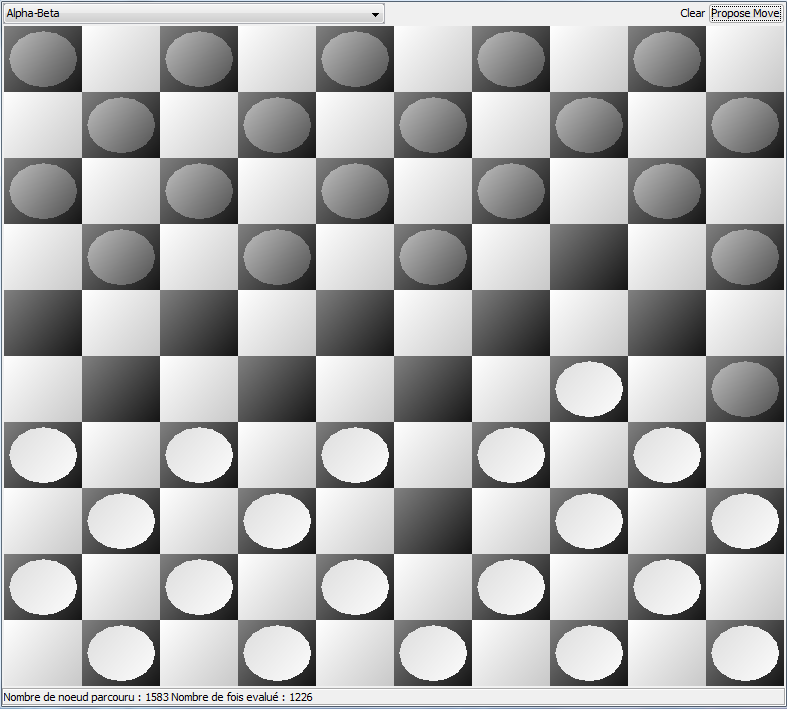
\includegraphics[scale=0.5]{img/screenshot_plateau.png}
\end{center}
\caption{Capture d'écran de l'interface du jeu}
\end{figure}

	\newpage
		
	\section{Algorithme du Min-Max}
	Une fois le jeu de dames implémenté, nous avons récupéré l'algorithme du min-max d'un ancien projet que l'un de nous avait réalisé. Il a fallu qu'on adapte l'algorithme, car au départ, il n'était pas générique. Nous l'avons donc rendu générique, pour pouvoir le réutiliser par la suite.\\
	
	\section{Algorithme Alpha-Béta}
	L'algorithme de l'Alpha-Beta a aussi été récupéré dans l'ancien projet. Nous l'avons aussi adapté en rendu générique.\\
	
		\section{Fonction d'évaluation}
	Pour pouvoir déterminer les nœuds les plus prometteurs, lors du parcours de l'arbre, nous avons codé une fonction d'évaluation. Celle-ci est utilisée par les deux algorithmes utilisés, à savoir le Min-Max, et l'Alpha-Béta.\\
	
	Notre fonction d'évaluation est calculée en fonction des critères suivants : 

	\begin{itemize}
		\item Le nombre de pions qu'il reste à chaque joueur. On l'appelle le critère matériel (mat).
		
		\item Le nombre de coups possibles pour chaque joueur. On l'appelle le critère de mobilité (mob). 
		
		\item Le nombre de pions qui sont ou qui vont entrer dans la zone gagnante. C'est-à dire dans la zone de l'adversaire. Ce critère est appelé position (pos)\\
\end{itemize}
	
  Ainsi, on définit notre fonction d'évaluation par un polynôme tel que :\\
	
	
	
	\begin{math}
 P_{mat}C_{mat} + P_{mob}C_{mob} + P_{pos}C_{pos}\\ 
	\end{math}
	\\
	Dans chacun des termes, on repère un coefficient, qui nous permet de déterminer l'importance de chaque paramètre. En d'autres termes, plus le coefficient multiplié à un critère calculé est élevé, plus le critère est important.
	
	
	\newpage
	
	\section{Apprentissage et Mémorisation}
	\subsection{Sauvegarde et Chargement des données}
	Finalement, nous avons implémenté un système de mémorisation des parties précédentes. Nous enregistrons les parties dans des fichiers textes. Ces fichiers textes sont enregistrés à l'endroit où se trouve l'exécutable du projet, ou sur Eclipse, à la racine du projet. Le nom de ces fichiers est constitué en utilisant la date et l'heure à laquelle l'enregistrement a été fait. 
	
	\begin{figure}[h]
\begin{center}
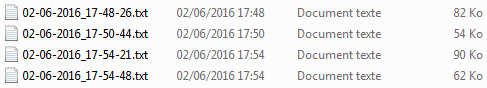
\includegraphics{img/screenshot_fichierstextes.png}
\end{center}
\caption{Capture d'écran de fichiers de parties sauvegardées}
\end{figure}
	
	On remarque sur nos fichiers textes, qu'ils n'ont pas tous la même taille. C'est dû au fait que suivant la partie, on ne sauvegarde pas le même nombre d'états du plateau.\\
	
	Dans ces fichiers textes, chaque ligne correspond à un état du plateau de jeu (un tableau à deux dimensions, en somme). Sur chacune de ces lignes, pour chaque case du plateau, on a un chiffre suivi de deux points, suivi d'un autre chiffre. Le premier chiffre correspond à la couleur du pion sur la case en question :\\
	
	\begin{itemize}
		\item -1 : C'est une case vide. Aucun pion n'est placé dessus.
		\item 0  : C'est un pion noir qui se trouve sur cette case.
		\item 1  : C'est un pion blanc qui se trouve sur la case.\\
	\end{itemize}
	
	Les deux points suivants servent de séparateur entre les deux chiffres, pour dire qu'ils vont ensemble. Enfin, le deuxième chiffre correspond au sens de direction du pion : \\
	
	\begin{itemize}
	\item 0 Le pion se déplace vers le bas.
	\item 1 Le pion se déplace vers le haut.
	\end{itemize}
	\newpage
	Nous avons décidé de sauvegarder l'état du pion, comme nous avions décidé de ne pas implémenter les pions et de leur faire faire demi-tour, à la place. Par conséquent, pour que l'ordinateur se rappelle d'une façon réaliste le plateau précédent, il fallait garder le sens des pions.

	\begin{figure}[h]
\begin{center}
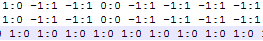
\includegraphics{img/screenshot_etats.png}
\end{center}
\caption{Capture d'écran des lignes dans un fichier}
\end{figure}	
	
	On remarque sur la figure 1.3 que la dernière ligne contient le même chiffre, c'est parce que la dernière ligne du fichier correspond à un plateau de même taille que les précédents, mais avec la couleur du gagnant, en premier chiffre.\\
	
	Ainsi, prenons par exemple un état d'une case pour exemple, l'état 0:0. Cet état signifie que c'est un pion noir, et qu'il se déplace vers le bas.\\
	\newpage
\subsection{Recherche et utilisation des états mémorisés}
Les fichiers nous permettent de construire un arbre de mémorisation. Chaque noeud de l'arbre représente un état du jeu (un plateau). Une fois cet arbre construit, nous appliquons un algorithme qui permet de récupérer les points de non retour des parties perdantes, pour un joueur qui utilise les pions noirs ou les pions blancs. \\

\begin{figure}[h]
\begin{center}
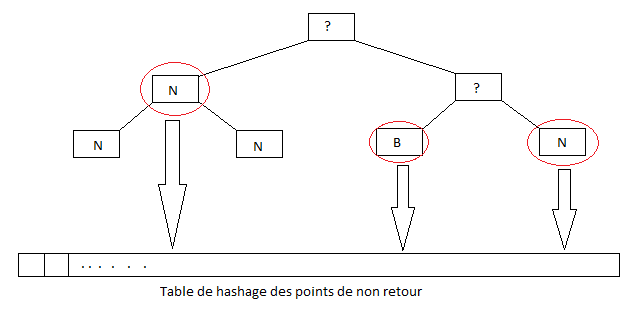
\includegraphics[scale=0.5]{img/arbre_hashage_memoire.png}
\end{center}
\caption{Schéma explicatif de l'utilisation de notre mémoire}
\end{figure}	

L'algorithme consiste à descendre jusqu'en bas de l'arbre et récupérer le pion perdant. En remontant dans l'arbre, on compare les fils de chaque noeuds. Si les deux fils sont égaux, on remonte la couleur du pion. Sinon, on remonte -1 et on enregistre tous les enfants qui ne sont pas égaux à -1. Cela nous donne les points de non retour possibles. Ces points de non retour sont enregistrés dans une table de hashage. Cette table est réutilisée dans l'algorithme Alpha-Beta, pour élaguer davantage l'arbre de décisions.\\


L'algorithme de calcul de la clé de hashage réalise une opération sur chaque case du plateau. Cette opération est la suivante :\\

Premièrement, chaque couleur de chaque case prend une nouvelle valeur (appelons cette valeur x) :\\
\begin{itemize}
\item -1 => 0
\item 0 => 2
\item 1 => 3
\end{itemize}
\newpage
Ensuite, pour chaque case, on incrémente un compteur élevé à la puissance x ( x étant la nouvelle valeur correspondante à une couleur) :\\

	\begin{math}
	\sum_{i=0}^{9}\sum_{j=0}^{9} (ij^{x})\\
	\end{math}
	
	\section*{Conclusion}
	Ce projet nous a permis de mettre en oeuvre les algorithmes vus en cours, et ainsi de les comprendre. Nous pensons que nous pourrions améliorer notre projet, tout d'abord en implémentant la transformation d'un pion en Reine, et aussi en réalisant un élagage de l'arbre de la mémoire. En effet, nous avons remarqué que nous enregistrons certaines parties, alors qu'elles n'ont pas vraiment lieu d'être enregistrées.
\end{document}